\documentclass[12pt,a4paper]{article}
\usepackage[utf8]{inputenc}
\usepackage{amsmath}
\usepackage[brazilian]{babel} % Brazil or not Brazil??
\usepackage{amsfonts}
\usepackage{amssymb}
\usepackage{graphicx}
\usepackage[margin=0.8in]{geometry}


\begin{document}
\title{\vspace{70mm}\Huge Experimento 06a - Calorimetria}
\author{ Giovani Garuffi\qquad\hfill
		\textit {RA: 155559}\protect\\
		João Baraldi\hfill
		\textit{RA: 158044}\protect\\
		Lauro Cruz\hfill
		\textit{RA: 156175}\protect\\
		Lucas Schanner\hfill
		\textit{RA: 156412}\protect\\
		Pedro Stringhini\hfill
		\textit {RA: 156983}								
		}
\maketitle
\newpage
\section{Resumo}
Neste experimento estudamos o calorímetro, um instrumento utilizado na medição de processos que envolvam trocas de calor.
O experimento está divido em duas partes, e a primeira será cobrida por este relatório. Os processos desta parte do experimento são divididas em três partes. Primeiramente, utilizando um termopar, colocamos uma de seus fios na água em temperatura de fusão e o outro fio em água em temperatura de ebulição e medidos pares de voltagem com a temperatura da água quente, traçando assim o gráfico de calibração do termopar.
Em uma segunda parte, calculamos a constante de tempo do calorímetro, preenchendo o calorímetro com água aquecida e com o calorímetro fechado, cronometra-se o tempo com que a temperatura cai.
Na terceira parte, obtemos a capacidade térmica do calorímetro enchendo metade do calorímetro com água a 18 $^{\circ}C$ e depois preenchendo-o com água a 82 $^{\circ}C$ , esperando assim o sistema entrar em euqilíbrio.

\section{Objetivos}
Este experimento pode ser divido em três partes, cada uma com seus objetivos, que são: traçar um gráfico de calibração de um termopar, calcular a constante de tempo de um calorímetro e calcular sua capacidade térmica.


\section{Procedimento Experimental e Coleta de Dados}


\subsection{Procedimento}


\subsubsection{Curva de calibração de um termopar}

  Nesta parte do experimento preenche-se uma parte do copo do calorímetro (vide figura \ref{calorimetro}) com água fervente e coloca-se nele um termômetro de mercúrio para controle de sua temperatura. Em um béquer separado, coloca-se água com gelo para manter sua temperatura próxima a zero.\\

\begin{figure}[!htbp]
\centering
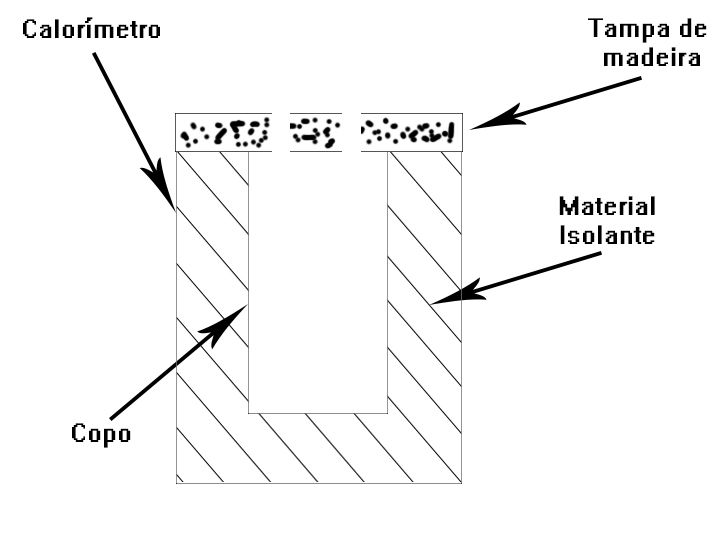
\includegraphics[scale=0.3]{Fig6a1.jpg}
\caption{Estrutura de um calorímetro.}
\label{calorimetro}
\end{figure}

Então, coloca-se o fio de referência do termopar dentro do copo com gelo e o outro fio dentro do calorímetro(como mostrado na figura \ref{exptermopar}). Então, adiciona-se água à temperatura inicial (retirada da torneira) no calorímetro, e, para cada temperatura da água do calorímetro lê-se uma voltagem (em $mV$) no termopar, anota-se a temperatura e a voltagem, até que primeira se aproxime da inicial.

\begin{figure}[!htbp]
\centering
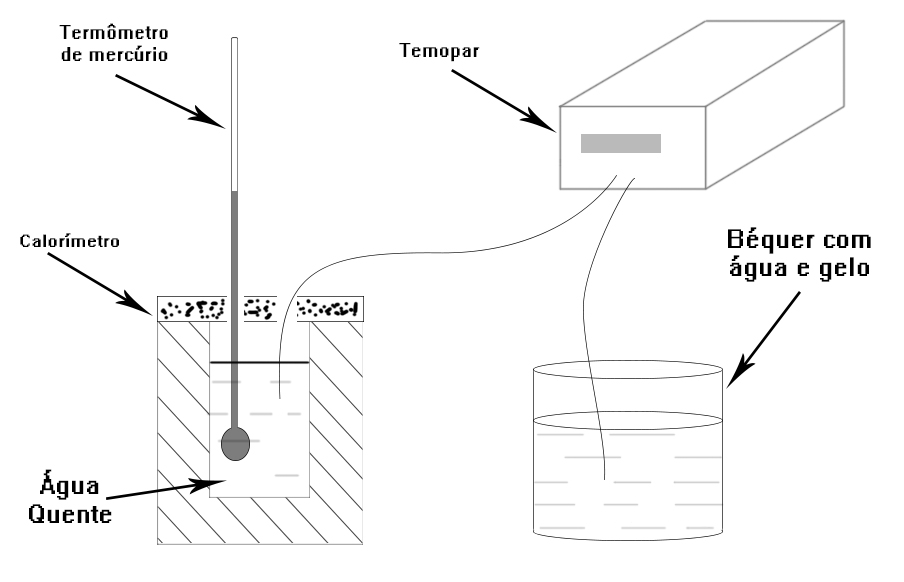
\includegraphics[scale=0.3]{Fig6a2.jpg}
\caption{Montagem experimental para a calibração do termopar.}
\label{exptermopar}
\end{figure}

Por fim, plota-se um gráfico $V \; x \; T$ com os pares anotados, e um com os tabelados teóricos.\\

\subsubsection{Constante de tempo de um calorímetro}

Como o calorimetro usado não é ideal, nesta parte do experimento, será calculada a sua constante de tempo, que representa a velocidade com que o calorímetro permite trocas de calor com o ambiente.\\
Para tal, prenche-se o calorimetro com água, que deve ser aquecida utilizando-se um ebulidor, e, com ele totalmente fechado (figura \ref{calorimetro}), mas com um termômetro dentro, cronometra-se o tempo com que a temperatura cai. No caso, foi medido o tempo de $T = 89 \; ^{\circ} C$ a $T = 69 \; ^{\circ} C$.\\
Então, pela fórmula 
$$T = T_0 e ^{-t/\tau} + T_a,$$
onde $T_0$ é a temperatura inicial, $t$ é o tempo, $\tau$ é a constante a ser encontrada e $T_a$ é a temperatura ambiente (de $26.5 ^{\circ}$, no caso), calcula-se o valor da constante através de um gráfico $ln(T) \; x \; t$.


\subsubsection{Capacidade térmica de um calorímetro}
Para determinar a capacidade térmica do calorímetro, metade do calorímetro foi enchida de água a temperura $18$ graus celsius. Depois, acrescentou-se a mesma quantidade de água quente a $82$ graus celsius, esperando o sistema entrar em equilibrio e vendo sua temperatura final $61$ graus celsius. Assim, a partir da relação:
$$-Q_{perdido H_2O} = Q_{recebido H_2O} + Q_{recebido Calorimetro}$$
$$-m_{H_2O_{quente}}\cdot c_{H_2O} \cdot (\theta_{final}-\theta_{quente}) = m_{H_2O_{fria}}\cdot c_{H_2O} \cdot (\theta_{final}-\theta_{frio}) + C_{cal}\cdot (\theta_{final}-\theta_{frio}) $$
$$C_{cal} = \frac{m_{H_2O_{quente}}\cdot c_{H_2O}\cdot(\theta_{quente} - \theta_{final}) + m_{H_2O_{fria}}\cdot c_{H_2O}\cdot(\theta_{frio} - \theta_{final})}{(\theta_{final}-\theta_{frio})},$$
Determina-se a capacidade térmica desejada.


\subsection{Dados Obtidos}

A Tabela \ref{dadostermopar} apresenta as medições Da tensão medida no termopar, em função da temperatura. Enquanto na Tabela \ref{dadostempo} estão presentes os
dados da tendência de queda de temperatura do calorímetro utilizado.

\newpage
\begin{table}[!htbp]

\centering
\def\arraystretch{1.5}
\caption{Medições de temperatura relacionadas a tensão medida em um termopar}

\begin{tabular}{|r|r|}
\hline
Tensão $(mV)$ & Temperatura $(C)$\\
\hline
 4.62 & 89 \\
 \hline
 4.40  & 87 \\
 \hline
 4.19 & 84 \\
 \hline
 3.96 & 80 \\
 \hline
 3.82 & 78 \\
 \hline
 3.04 & 65 \\
 \hline
 2.89 & 62 \\
 \hline
 2.44 & 54 \\
 \hline
 2.31 & 51 \\
 \hline
 2.03 & 47 \\
 \hline
 1.94 & 45 \\
 \hline
 1.80  & 42 \\
 \hline
 1.69 & 40 \\
 \hline
 1.44 & 37 \\
\hline
\end{tabular}

\emph{O erro na temperatura é de $0.5 C$, e na tensão de $0.01 mV$}
\label{dadostermopar}
\end{table}

\begin{table}[!htbp]

\centering
\def\arraystretch{1.5}
\caption{Medidas de temperatura de um calorímetro}

\begin{tabular}{|r|r|}
\hline
Tempo $(s)$ & temperatura $(C)$ \\
\hline
    0 & 89 \\    
  700 & 78 \\
  860 & 76 \\
 1500 & 71 \\
 1610 & 70 \\
\hline
\end{tabular}

\emph{O erro na temperatura é de $0.5 C$, e no tempo de $0.5 s$}
\label{dadostempo}
\end{table}


\section{Análise dos Resultados e Discussões}

\subsection{Curva de Calibração do Termopar}
Para comparar os dados obtidos no experimento e os dados conhecidos de tensão em função da temperatura, foi construído o gráfico na Figura \ref{termopar}.  \\
Verifica-se que houve algum tipo de erro experimental na realização, uma vez que os resultados obtidos são internamente consistentes (A relação é linear, assim como esperado), mas existe uma diferença significativa das medidas esperadas.

% INSERT migués HERE 
 
\begin{figure}[!htbp]
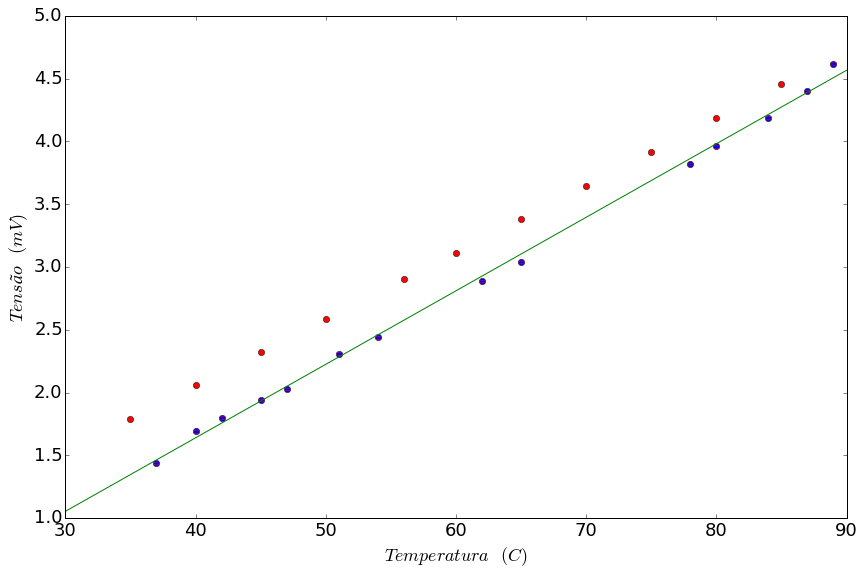
\includegraphics[scale=0.55]{termopar.png}
\caption{Curva de calibração do termopar. As medidas Azuis são as obtidas experimentalmente e as vermelhas são as esperadas}
\label{termopar}
\end{figure}

Esse deslocamento da reta, foi, provavelmente, resultado de erros sistemáticos como uma temperatura de referência diferente de $0 \; ^{\circ} C$.

\subsection{Constante de tempo do calorímetro}
A queda de temperatura da agua no calorímetro pode ser descrita pela equação
$$ T = T_0 e^{-t/\tau} + T_a $$
que pode ser reescrita como
$$ \ln \Delta T = -t/\tau + \ln T_0 $$
Vemos então que deve haver uma relação linear entre $ln \Delta T$ e $ t $. Para verificar essa relação foi construido a tabela \ref{table:tempo} e o gráfico da figura \ref{fig:tempo}. \\
\begin{table}[!htbp]
\centering
\def\arraystretch{1.5}
\caption{Dados relacionando $ln \Delta T$ à $t$}
\label{table:tempo}
\begin{tabular}{|c|l|r|r|}
\hline
Temperatura $\; (C)$ & $\Delta T \; (C)$ & $\ln \Delta T \; (\ln C)$ & tempo $\; (s)$ \\
\hline
 $89 \pm 0.5$ & $ 62.5 \pm  0.7 $ & $ 4.135 \pm 0.008 $    &    0 \\
 \hline
 $78 \pm 0.5$ & $ 51.5 \pm  0.7 $ & $ 3.941 \pm 0.009 $ &  700 \\
 \hline
 $76 \pm 0.5 $& $ 49.5 \pm  0.7 $ & $ 3.90 \pm 0.01 $ &  860 \\
 \hline
 $71 \pm 0.5$ & $ 44.5 \pm  0.7 $ & $ 3.79 \pm 0.01 $ & 1500 \\
 \hline
 $70 \pm 0.5$& $ 43.5 \pm  0.7 $ & $ 3.77 \pm 0.01 $ & 1610 \\
\hline
\end{tabular}\\
\emph{$\Delta T$ for calculado a partir de uma temperatura ambiente de $26.5 C$}

\end{table}
Fazendo a regressão linear sobre os dados da tabela \ref{table:tempo}, obtemos os coeficientes 
$$ a = -0.000232 \pm 0.000007\qquad e\qquad b = 4.125 \pm 0.007 $$

\begin{figure}[!htbp]
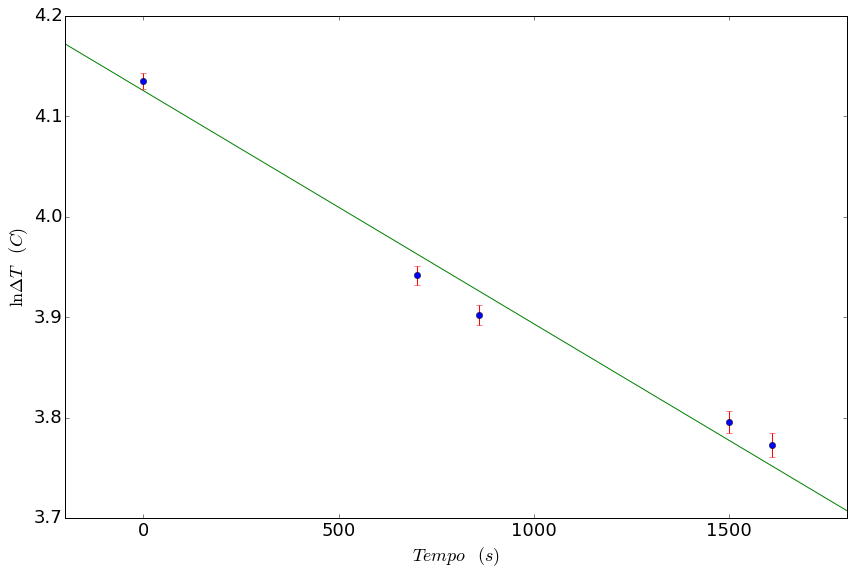
\includegraphics[scale=0.55]{tempo.png}
\caption{Gŕafico de regressão linear de $ \ln \Delta T$ por $t$.}
\label{fig:tempo}
\end{figure}

Sabemos então que, pela relação $ \ln \Delta T = -t/\tau + \ln T_0 $, $a = -\frac{1}{\tau}$ e, portanto:
$$ \tau = -\frac{1}{a}; $$
$$ \Delta\tau =\frac{\Delta a}{a^2}. $$
Assim, 
$$ \tau = (4300 \pm 100)s $$
\subsection{Capacidade termica do calorímetro}

A partir da fórmula $$C_{cal} = \frac{m_{H_2O_{quente}}\cdot c_{H_2O}\cdot(\theta_{quente} - \theta_{final}) + m_{H_2O_{fria}}\cdot c_{H_2O}\cdot(\theta_{frio} - \theta_{final})}{(\theta_{final}-\theta_{frio})},$$
sabemos calcular a capacidade térmica do caloímetro.
A massa de água quente é de $(133,3 \pm 0,1)g$ com temperatura $(49,0 \pm 0,5)^{\circ}\mathrm{C}$, e a massa de água fria é $(137,3 \pm 0,1)g$, com temperatura $(35,0 \pm 0,5)^{\circ}\mathrm{C}$.

Sabendo que a temperatura de equilíbrio é $(41,0 \pm 0,5)^{\circ}\mathrm{C}$, tem-se que:
$$C_{cal} = 40,43 \,^{\circ}\mathrm{C}^{-1}. $$

\section{Conclusões}
O experimento obteve sucesso em descrever a curva de calibração de um termopar com razoável precisão. Houve uma discrepância com os dados esperados que pode ser explicada pela diferença na temperatura de referência.\\
Também foi possível obter a constante de tempo do calorímetro como $4300 \pm 100 (s)$ .

\end{document}

